\documentclass[12pt]{article}
\usepackage{tikz}

\begin{document}
%% 线条样式
\section{Line Style}
\begin{tikzpicture}
    % 绘制箭头
    \draw [->] (0, 0) -- (2, 0);
    \draw [<-] (0, -0.5) -- (2, -0.5);
    \draw [|->] (0, -1) -- (2, -1);
    \draw [<->] (0, -2) -- (0, -4) -- (3, -4);
\end{tikzpicture}

\vspace{2cm}

% 调整线条粗细

\begin{tikzpicture}
    \draw [ultra thick] (0, 3) -- (3, 3);
    \draw [very thick] (0, 2.5) -- (3, 2.5);
    \draw [thick] (0, 2) -- (3, 2);
    \draw [semithick] (0, 1.5) -- (3, 1.5);
    \draw [thin] (0, 1) -- (3, 1);
    \draw [very thin] (0, 0.5) -- (3, 0.5);
    \draw [ultra thin] (0, 0) -- (3, 0);
\end{tikzpicture}

\vspace{2cm}

%% 其他线条样式

\begin{tikzpicture}
    % 自定义线条粗细
    \draw [line width=3] (0, 1) -- (3, 1); % 默认单位是 pt
    \draw [line width=0.2cm] (0, 0.5) -- (3, 0.5);
    \draw [line width=3mm] (0, 0) -- (3, 0);
\end{tikzpicture}

\vspace{1cm}

\begin{tikzpicture}
    % 虚线
    \draw [dashed, ultra thick] (0, 1) -- (3, 1); 
    \draw [dashed] (0, 0.5) -- (3, 0.5);
    \draw [dotted] (0, 0) -- (3, 0);
\end{tikzpicture}

\vspace{1cm}

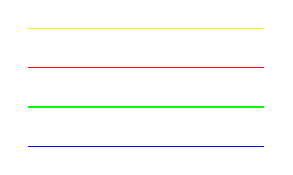
\begin{tikzpicture}
    % 颜色
    \draw [yellow] (0, 1.5) -- (3, 1.5);
    \draw [red] (0, 1) -- (3, 1); 
    \draw [green] (0, 0.5) -- (3, 0.5);
    \draw [blue] (0, 0) -- (3, 0);
\end{tikzpicture}

\newpage

%% 节点
\section{Node}
% shape声明节点形状, draw声明边框颜色, fill声明填充颜色, thick声明边框线宽
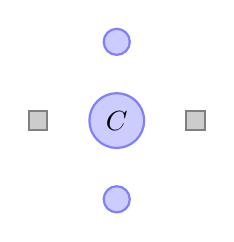
\begin{tikzpicture}
    \tikzstyle{aaa} = [shape=circle, draw=blue!50, fill=blue!20, thick]
    \tikzstyle{bbb} = [shape=rectangle, draw=black!50, fill=black!20, thick] 
    % 第一种节点命名方式 
    \path   (0, 2) node [aaa, name=a1] {} 
            (0, 1) node [aaa, name=a2] {$C$}
            (0, 0) node [aaa, name=a3] {}
            (1, 1) node [bbb, name=b1] {}
            (-1, 1) node [bbb, name=b2] {};

    % % 第二种节点命名方式
    % \node (a1) [aaa] at (0, 2) {}; 
    % \node (a2) [aaa] at (0, 1) {$C$};
    % \node (a3) [aaa] at (0, 0) {};
    % \node (b1) [bbb] at (1, 1) {};
    % \node (b2) [bbb] at (-1, 1) {};
\end{tikzpicture}

\vspace{2cm}
% 基于相对位置绘制节点: above of, below of, left of, right of
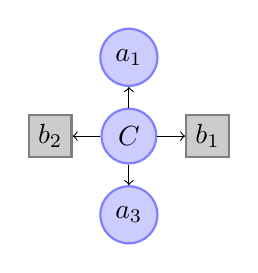
\begin{tikzpicture}
    \tikzstyle{aaa} = [shape=circle, draw=blue!50, fill=blue!20, thick]
    \tikzstyle{bbb} = [shape=rectangle, draw=black!50, fill=black!20, thick]  
    \node (a1) [aaa]                 {$a_1$};
    \node (a2) [aaa] [below of = a1] {$C$};
    \node (a3) [aaa] [below of = a2] {$a_3$};
    \node (b1) [bbb] [right of = a2] {$b_1$};
    \node (b2) [bbb] [left of = a2]  {$b_2$};
    
    % 使用east, west, north, south, center声明位置连接节点
    \draw [->] (a2.west) -- (b2.east);
    \draw [->] (a2.east) -- (b1.west);
    \draw [->] (a2.north) -- (a1.south);
    \draw [->] (a2.south) -- (a3.north);

    % % 利用相对位置连接节点,不声明连接位置
    % \draw [->] (a2) -- (b2);
    % \draw [->] (a2) -- (b1);
    % \draw [->] (a2) -- (a1);
    % \draw [->] (a2) -- (a3);
\end{tikzpicture}

\vspace{2cm}
% 利用edge命令连接节点
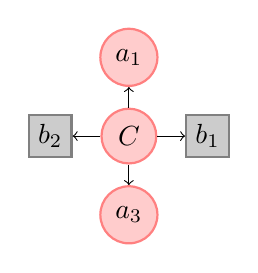
\begin{tikzpicture}
    \tikzstyle{aaa} = [shape=circle, draw=red!50, fill=red!20, thick]
    \tikzstyle{bbb} = [shape=rectangle, draw=black!50, fill=black!20, thick]  
    \node (a1) [aaa]                 {$a_1$};
    \node (a2) [aaa] [below of = a1] {$C$} edge [->] (a1);
    \node (a3) [aaa] [below of = a2] {$a_3$} edge [<-] (a2);
    \node (b1) [bbb] [right of = a2] {$b_1$} edge [<-] (a2);
    \node (b2) [bbb] [left of = a2]  {$b_2$} edge [<-] (a2);

    % % 利用edge连接节点的第二种方式
    % \path   (0, 2) node [aaa, name=a1] {$a_1$} 
    %         (0, 1) node [aaa, name=a2] {$C$} edge [->] (a1)
    %         (0, 0) node [aaa, name=a3] {$a_3$} edge [<-] (a2)
    %         (1, 1) node [bbb, name=b1] {$b_1$} edge [<-] (a2)
    %         (-1, 1) node [bbb, name=b2] {$b_2$} edge [<-] (a2);
\end{tikzpicture}

\vspace{2cm}
% 周围节点连接线穿过中心点
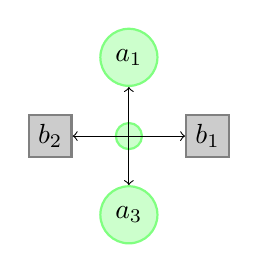
\begin{tikzpicture}
    \tikzstyle{aaa} = [shape=circle, draw=green!50, fill=green!20, thick]
    \tikzstyle{bbb} = [shape=rectangle, draw=black!50, fill=black!20, thick]  
    \node (a1) [aaa]                 {$a_1$};
    \node (a2) [aaa] [below of = a1] {};
    \node (a3) [aaa] [below of = a2] {$a_3$};
    \node (b1) [bbb] [right of = a2] {$b_1$};
    \node (b2) [bbb] [left of = a2]  {$b_2$};

    \draw [->] (a2.center) -- (b2.east);
    \draw [->] (a2.center) -- (b1.west);
    \draw [->] (a2.center) -- (a1.south);
    \draw [->] (a2.center) -- (a3.north);
\end{tikzpicture}
\end{document}